%% LyX 2.0.4 created this file.  For more info, see http://www.lyx.org/.
%% Do not edit unless you really know what you are doing.
%\documentclass[11pt,oneside,english]{amsart}
\documentclass[11pt,english]{article}
\usepackage[T1]{fontenc}
\usepackage[latin9]{inputenc}
\usepackage{geometry}
\geometry{verbose, margin = 1in}
\usepackage{amsthm}
\usepackage{amsmath}
\usepackage{tikz}
\usepackage{array}
\usetikzlibrary{arrows}
\usepackage{subfigure}

\setlength{\parskip}{0.63pc}

% Split long \texttt (now \path) lines
\usepackage{url}


\makeatletter
%%%%%%%%%%%%%%%%%%%%%%%%%%%%%% Textclass specific LaTeX commands.
%\numberwithin{equation}{section}
%\numberwithin{figure}{section}
\theoremstyle{plain}
\newtheorem{thm}{\protect\theoremname}
  \theoremstyle{definition}
  \newtheorem{defn}[thm]{\protect\definitionname}
  \theoremstyle{plain}
  \newtheorem{lem}[thm]{\protect\lemmaname}

\makeatother

\usepackage{babel}
  \providecommand{\definitionname}{Definition}
  \providecommand{\lemmaname}{Lemma}
\providecommand{\theoremname}{Theorem}

\begin{document}

\title{Text Indexing with Wildcards: An Experimental Comparison \\[0.15in]
	\large{\textsc{6.851 Final Project}}
	\vspace{-2pt}
	}
\author{Hayden Metsky (hmetsky@mit.edu) and Casey O'Brien (cmobrien@mit.edu)}
\date{\vspace{-15pt}May 18, 2014}

\maketitle


\section{Introduction}

Consider the text indexing problem. Given an input text and query string, we wish to report all the indices of the input text to which the query string matches. In this paper we will consider a generalized version of this problem, in which we allow the query string to contain \textit{wildcards}. A wildcard is a character which can be matched to any other character. We will discuss four possible approaches to this problem. The first two are naive solutions, one of which uses little space but has a slow query time, and the other which has a fast query time but uses a lot of space. Then, we discuss two approaches presented by Cole et al. in 2004 \cite{cole}.

While theoretical bounds for each of these solutions have already been established, our goal is to report the performance of each of these solutions in practice. To this end, we implemented each of them in Java. For each solution, we measure the total space and query time for various texts and query patterns, allowing varying numbers of wildcards.

In terms of space, the solutions perform as expected based on their theoretical bounds. Perhaps more interestingly, the actual query time performance of the query algorithms differ substantially from what we expected based on their theoretical runtimes. In particular, the full structure and final solution developed by Cole et al. performs worse in query time than both naive approaches, and also performs worse than a watered-down, introductory solution offered by Cole et al.

\subsection{Organization of the Report}

In section~\ref{sec:survey} we present an overview of each of the solutions as well as their theoretical bounds. In Section~\ref{sec:methodology}, we discuss the details of the implementation of our structures and the methods we used to measure their performance. In Section~\ref{sec:results}, we present the results of our experimentation, and finally in section~\ref{sec:discussion} we discuss the underlying reasons for and implications of these results.

\subsection{Notation}

Throughout this paper, for ease of notation, we will interchangeably use $t$ to refer to the query text itself and also the length of the query text (and similarly for $p$). We will use $k$ to denote the maximum number of wildcards allowed in a query. Note that because the building of the structures can depend on $k$, we require that this parameter be set beforehand and not dynamically with each query. We will use $\Sigma$ to denote the size of the alphabet. Finally, we will use the symbol $*$ to denote a wildcard.

\begin{figure*}[!t]
\begin{center}
\fbox{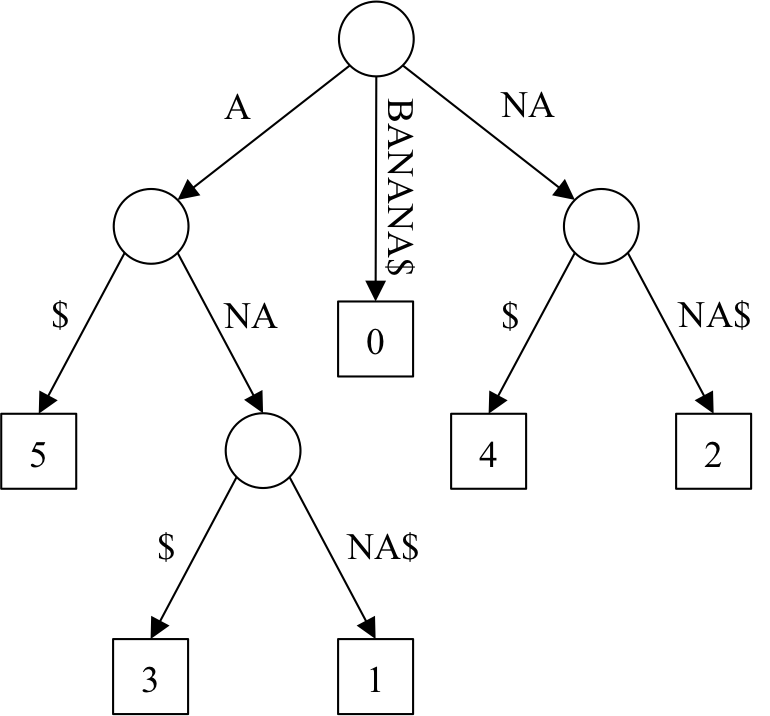
\includegraphics[height = 2in]{figures/banana.png}}
\fbox{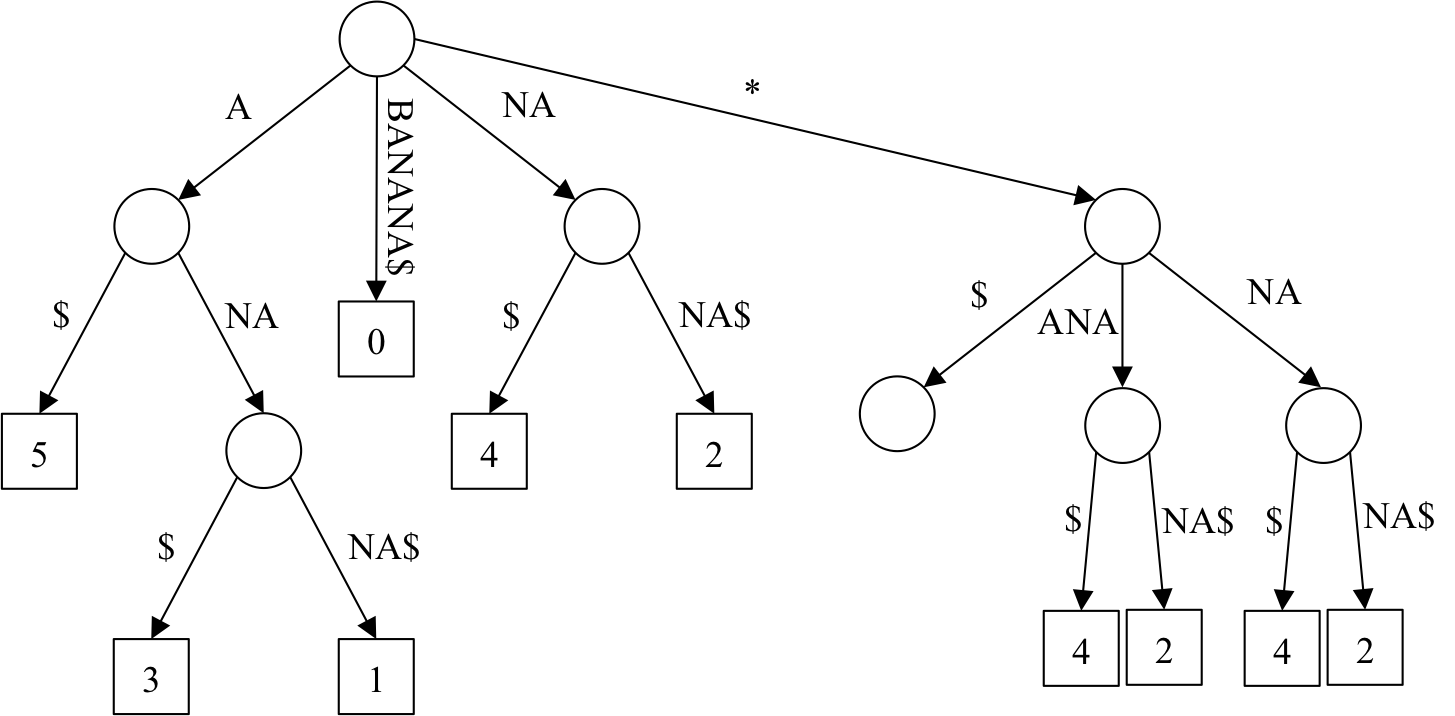
\includegraphics[height = 2in]{figures/bigspace.png}}
\end{center}
\label{fig:sample}
\caption{\small{On the left is the standard suffix tree for $t =$ BANANA. On the right, the suffix tree has been modified to contain a wildcard subtree at the root. Note that the big space, fast query solution requires wildcard subtrees be created between every letter.}}
\end{figure*}


\section{Survey of Solutions to the Text Indexing Problem}
\label{sec:survey}

\subsection{Naive Solution 1: Small Space, Slow Query}

This solution uses only a standard suffix tree $S$ on $t$. To perform the query, we perform a standard query on the suffix tree, with the addition that each time we come across a wildcard in $p$, we branch and explore all possible subtrees. The space for this solution is clearly $O(t)$, and the time for a query is $O(\Sigma^kp + \text{\# match})$, where $\text{\# match}$ is the number of matches of the query. The $\Sigma^k$ term arises from the fact that we may have to fully explore every subtree of a node each time we reach a wildcard. We will refer to this solution as the \textsc{Slow-Query} approach.

\subsection{Naive Solution 2: Big Space, Fast Query}

By modifying the suffix tree to store additional information, we can achieve a much faster query time. For this solution, we modify each node $v$ to contain an edge to a wildcard subtree. This edge will represent the wildcard. We build a suffix tree from all the suffixes represented below $v$, skipping over the first letter of each suffix. We build these wildcard subtrees recursively, such that each root-to-leaf path contains at most $k$ wildcards. Note that building these subtrees involves splitting edges, because we need to have the option to match a wildcard instead of any given letter. Figure~\ref{fig:sample1} shows an example suffix tree with a single wildcard tree built. With these wildcard subtrees, we have a query time of $O(p + \text{\# match})$. However, the space required to store this tree is $O(t^{1 + k})$.  We will refer to this solution as the \textsc{Big-Space} approach.


\begin{figure*}[!t]
\begin{center}
\fbox{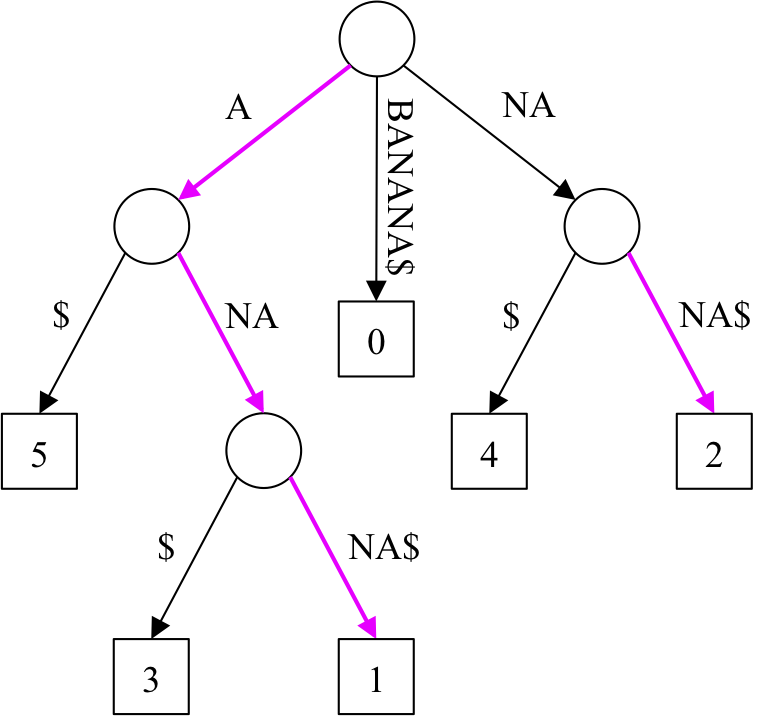
\includegraphics[height = 2in]{figures/centroid.png}}
\fbox{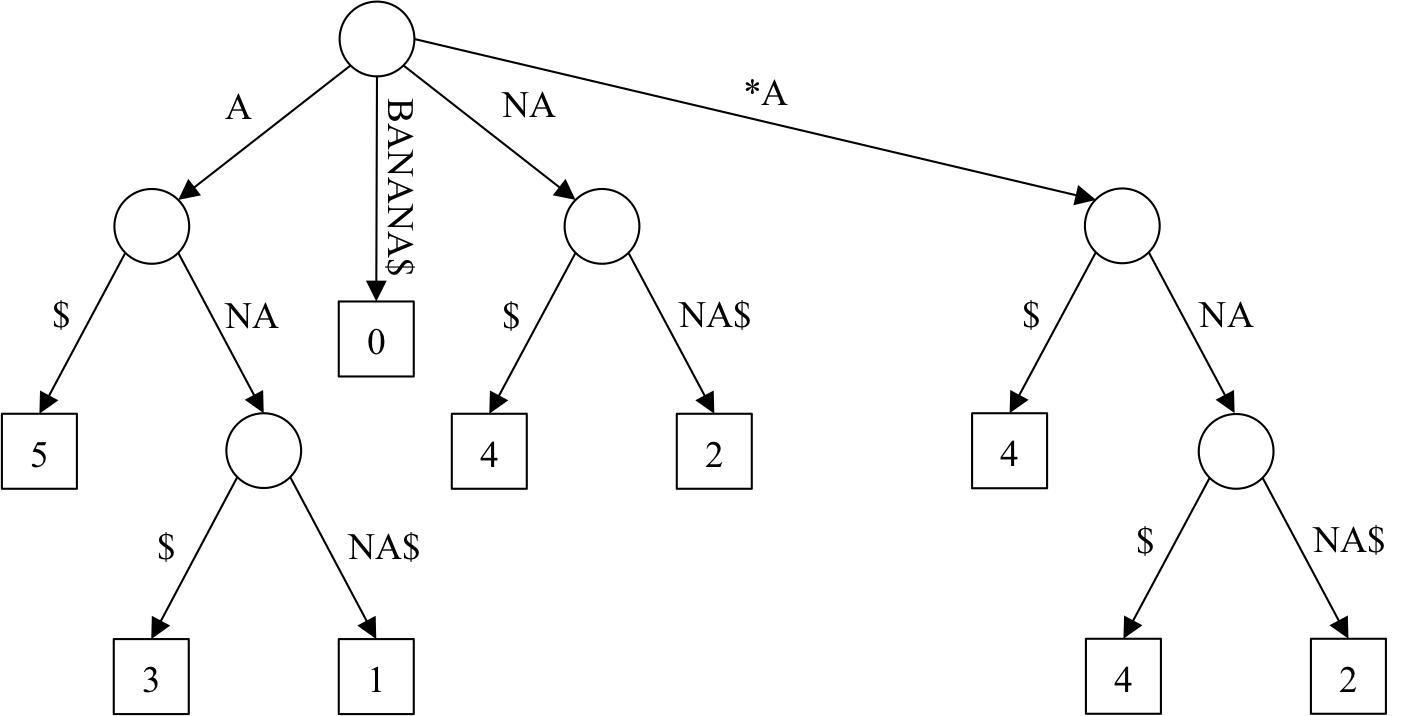
\includegraphics[height = 2in]{figures/wildcardcentroid.png}}
\end{center}
\label{fig:sample}
\caption{\small{On the left is the standard suffix tree for $t =$ BANANA, with centroid edges highlighted. On the right, the suffix tree has been modified to contain a CPD wildcard subtree at the root.}}
\end{figure*}

\subsection{Cole et al. Solution 1: Centroid Path Decomposition with Slow Query}
\label{subsec:cpdslow}

In 2004, Cole et al. provide a solution (that we call \textsc{CPD-Slow}) to this problem which achieves faster query time that the first solution, but less space than the second solution. In order to achieve this, the suffix tree is first decomposed into \textit{centroid paths}. The centroid path from the root to one of its descendant leaves is the path which follows the edges with the most descendant leaves (breaking ties arbitrarily). For nodes hanging off of this centroid path, centroid paths are created recursively. The centroid edge of a node is the outgoing edge of the node which lies along a centroid path. By construction, each node has exactly one centroid edge. Figure~\ref{fig:sample2} shows the centroid path decomposition of an example suffix tree.

Like the big space solution described above, the Centroid Path Decomposition (CPD) solution builds wildcard subtrees. However, the wildcard subtrees only include suffixes below the node which do not lie along the centroid edge of that node. With this construction, the space to store the suffix tree is only $O(t\log^k{t})$.

The general idea for the query is that whenever we reach a wildcard, we have to explore both the edge along the centroid path and the wildcard edge. Formally, to perform a query, we begin by dividing the query $p = p_0*p_1*\dots*p_k$, where each of the segments $p_i$ contain no wildcards. We begin by performing the following steps for $i = 0$, and continue until we have either finished with $i = k$ or have discovered a place where $p$ diverges from $t$.

\begin{enumerate}
\item Perform a standard query for $p_i$. Say that this query ends at position $v$ in the tree (which could be a node or along an edge).
\item If $v$ has depth equal to the length of $p_i$ below the starting point, then the query continues. Otherwise $p_i$ must diverge from $t$ and we return no matches.
\item If $v$ is a node:
\begin{enumerate}
\item Advance once character along the centroid path (to account for the wildcard), and then recurse from that location on $p_{i + 1}$.
\item Recurse from the root of the wildcard subtree rooted at $v$ on $p_{i + 1}$.
\end{enumerate}
\item Otherwise $v$ is a point along an edge. Advance one character along the edge and then recurse from that location on $p_{i + 1}$.
\end{enumerate}

If the query returns locations within the tree, we report all the leaf descendants of those locations as matches. For each wildcard, we might branch and explore two different edges. Thus, the total time for this query is $O(2^kp + \text{\# match})$.

\subsection{Cole et al. Solution 2: Centroid Path Decomposition with Fast Query}
\label{subsec:cpdfast}

In their paper, Cole et. al suggest a way (that we called \textsc{CPD-Fast}) to speed up the query time by using a carefully constructed longest common prefix (LCP) query instead of walking down the tree as we did in Step (1) above. The structure is the same as that described in the previous section. We will need to augment the tree with additional information, but we will be sure that the information never takes more than linear space in the size of the tree. Thus the space is still $O(t\log^k{t})$.

This new algorithm calls for preprocessing of $p$ which takes time $O(p)$. The LCP query takes time $O(\log\log{t})$. When we replace Step (1) from above with this LCP query, executing the entire query takes time $O(2^k \log\log{t} + \text{\# match})$. Thus, the overall time of the query will be $O(p + 2^k\log{\log{t}} + \text{\# match})$.

Let $S$ be the original suffix tree on $t$. In order to be able to answer LCP queries, we need to build some structures into our suffix tree. We will refer to these structures collectively as the LCP structure. An LCP structure needs to be built for each subtree hanging off a centroid path. All LCP structures are built as part of the preprocessing of the text.

Next we describe the LCP query. Formally, the LCP query takes a node $r$ and query text $p_i$ (with no wildcards), and returns the location $v$ which corresponds to the deepest location at which $p_i$ could be matched, starting at $r$. For now, we will assume that the subtree rooted at $r$ contains its own LCP structure. Because we don't build an LCP structure on every subtree, this may not actually be the case; after we describe the query, we will describe how to handle the case where $r$ is not at the root of some LCP structure.


Let $T$ be an arbitrary subtree on which we are building the LCP structure. First, the LCP structure on $T$ needs to be able to return the LCA (least common ancestor) of any two nodes in $T$. This can be done in space $O(|T|)$ with constant time queries using the techniques described in \cite{lec}.

Next, the LCP structure needs to support weighted level ancestor (WLA) queries. Given a node $v$ and a height $h$, a WLA query should return the position at height $h$ above $v$ in $T$. The (unweighted) level ancestor problem can be solved in constant time and $O(|T|)$ space \cite{lec}. The same ideas can be used to solve the weighted level ancestor problem, but the query time increases to $O(\log\log{t})$ due to the need to make a predecessor query.

Finally, each leaf in $T$ needs to store the index of its corresponding suffix in lexicographic order in $S$. We will refer to this value as $I_x$, where $l_x$ is some leaf node. Note that we store the index of this suffix in $S$, even though we are currently building a LCP structure on $T$. Then, given the index $I_x$ of a leaf, we need to return the two leaves in $T$ which have indices that are the predecessor and successor of $I_x$. This can be done in $O(\log\log{t})$ by storing the indices of all the leaves of $T$ in a $y$-fast trie.

Recall that we have divided $p$ into $p_0*p_1*\dots*p_k$. When we receive a query $p$, we perform the following preprocessing for each $p_i$. Our goal is to determine, for each $p_i$, the \textit{index} $g_i$ of $p_i$, and also the leaf with which $p_i$ has the most overlap. The index $g_i$ of $p_i$ is the lexicographic position that would be assigned to $p_i$ if it were in $S$. We determine this value as follows.

\begin{enumerate}
\item Proceed like a standard query in $S$ for $p_i$, noting the endpoint.
\item Compute the leaf $l_i$ corresponding to the closest string to $p_i$, lexicographically. This can be found easily as long as each node has a pointer to its leftmost and rightmost leaf descendants. Also store $h_i$, the length of the longest common prefix of the suffix on $l_i$ and $p_i$.
\item If the suffix at $l_i$ comes before $p_i$ lexicographically, $g_i = I_i + \frac{1}{2}$. Otherwise $g_i = I_i - \frac{1}{2}$.
\end{enumerate}

It takes $O(p_i)$ to perform the preprocessing for any given $p_i$, so the total time to perform the preprocessing is $O(p)$. Once we have completed the preprocessing, then we are prepared to complete an LCP query. The query is computed as described below.

\begin{enumerate}
 \item Look up the leaves in $T$ with lexicographic indices corresponding to the predecessor (call this $l_p$) and successor (call this $l_s$) of $g_i$. Each leaf should also store a pointer to the leaf in $S$ with the same index.
 \item Compute $h_p$, the depth of the node $LCA(l_p, l_i)$ in $S$, and symmetrically $h_s$ from $LCA(l_s, l_i)$.
 \item Compute $\max\{h_p, h_s\}$. Without loss of generality assume the maximum was $h_p$. All further steps are symmetric if $h_s$ is chosen.
 \item Compute $h = \min\{h_i, h_p\}$. The represents the amount of overlap between $p_i$ and $T$.
 \item Let $d_p$ be the depth of the predecessor. Return $WLA(l_p, d_p -h)$.
\end{enumerate}

Steps (1) and (5) take $O(\log\log{t})$ due to the structures described above, and Steps (2), (3), and (4) take constant time. Thus, the overall time to complete this query is $O(\log\log{t})$.

Finally, we need to handle the case where we want to perform an LCP query on a node $r$ which is not at the root of an LCP structure. To perform this query, we will carefully choose a descendant node which is the root of an LCP structure, and then perform the LCP query from there. Let $T$ be the subtree which is rooted at the nearest ancestor of $r$ with a LCP structure. We perform, as follows, an LCP query on a node that is not at the root of an LCP structure.

\begin{enumerate}
\item Let $C$ be the centroid path in $T$ which contains $r$ (each node stores a pointer to its centroid path).
\item Find the leaf $l_u$ in $S$ corresponding to the suffix represented by the portion of $C$ below $r$. To do so:
\begin{enumerate}
\item Get the offset in $t$ of the leaf in $T$ at the end of $C$ (each leaf stores this information).
\item The offset of $l_u$ in $t$ is equal to this offset plus the depth of $r$ in $T$.
\item Look up the leaf in $S$ corresponding to this offset (we can store a table of these pointers).\end{enumerate}
\item Compute $h'$ as the depth of node $LCA(l_u, l_i)$ in $S$.
\item Let $h = \min\{h_i, h'\}$.
\item Find the position $v$ at height $h$ below $r$ on $C$. To do this, for each centroid path we store a $y$-fast trie containing depths of all the nodes along $C$.
\item If $v$ is not a node, then return position $v$. Otherwise, perform another LCP query on the child of $v$ corresponding to the next letter of $p_i$. This child will be the root of an LCP structure since it is hanging off a centroid path.
\end{enumerate}

Steps (2), (5), and (6) take $O(\log\log{t})$, and steps (1), (3), and (4) can be done in constant time. Thus, we have an overall LCP query time of $O(\log\log{t})$ for any node.

Now we can perform a query by first preprocessing $p$, and then continuing with the steps outlined in Section~\ref{subsec:cpdslow}, with the modification that instead of performing a standard query in Step (1) we perform an LCP query. The overall time of this algorithm is then $O(p + 2^k \log\log{t} + \text{\# match})$.

\section{Methodology}
\label{sec:methodology}

\subsection{Implementation of the Approaches}
We implemented the four approaches in the Java programming language.
While other languages may yield better performance, our primary objective is to measure relative performance between the approaches rather than strive for an optimal absolute performance.
Java is the language with which we are most comfortable, and it was therefore a natural choice.

We began by implementing a standard suffix tree to support the \textsc{Slow-Query} approach\footnote{In our code, this is the \path{stringmatch.ds.suffixtree.SuffixTree} class.}.
Indeed, this is the simplest data structure because the structure itself has no recursion beyond what is in a typical trie; furthermore, the query is a straightforward recursive algorithm.
To construct the tree, we implemented Ukkonen's algorithm, which is an online algorithm that runs in $O(t)$ time.
Our implementation of the algorithm was based heavily on a StackOverflow post~\cite{ukkonenstackoverflow} and on an existing implementation~\cite{ukkonengithub}.
In fact, while we initially believed an online approach would be helpful for later components of the implementation, and thus chose this algorithm, it turned out to not be necessary; any linear-time algorithm for constructing a suffix tree would have sufficed.
Prior to constructing the tree, we read the input text once and store it once.
We built a collection of small structures\footnote{In our code, these are in the \path{stringmatch.ds.text} package.} to easily work with substrings of the text, where each substring is simply stored using pointers to the original text.
Thus, each edge can store a substring of the text with $O(1)$ space, as desired.

We then proceeded by generalizing the standard suffix tree to recursively build wildcard subtrees down to a depth of $k$ wildcards\footnote{In our code, this is the \path{stringmatch.ds.suffixtree.SuffixTreeNaiveBigSpace} class.}.
This enables us to support the \textsc{Big-Space} approach.
Like the \textsc{Slow-Query} approach, the queries in this approach are implemented in a relatively straightforward manner using recursion.

We modified the \textsc{Big-Space} data structure to support the \textsc{CPD-Slow} and \textsc{CPD-Fast} structures\footnote{In our code, this is the \path{stringmatch.ds.suffixtree.SuffixTreeeWithCPD} class.}.
Namely, when we build a wildcard subtree off a node $v$, we copy the entire subtree of $v$ except the part under its centroid edge.
We then devised and implemented an algorithm (that we call \path{condense}\footnote{In our code, this is implemented in the \path{stringmatch.ds.suffixtree.Node} class.}) that recompresses this subtree in linear-time.
One variant of this structure (\textsc{CPD-Slow}) simply stores these wildcard subtrees and supports queries as described in Section~\ref{subsec:cpdslow}.
It does not store any extra information with each wildcard subtree beyond what is necessary.
The second variant of the structure (\textsc{CPD-Fast}) associates with each wildcard subtree information that allow us to perform efficient LCP queries as described in Section~\ref{subsec:cpdfast}.

In particular, for this second variant we implemented from scratch, using 6.851 notes as reference, structures to support LCA queries and WLA queries, as well as a $y$-fast trie to support predecessor and successor queries on indices of a subtree.
We store these structures in each wildcard subtree\footnote{The LCA and WLA structures can be found directly in the \path{stringmatch.ds.suffixtree.SuffixTreeeWithCPD} class. The $y$-fast trie can be found in the \path{stringmatch.ds.suffixtree.yfasttrie} package.}.
In implementing each of these structures we needed to support worst-case constant-time lookup in a hash table.
To do this, we used a Java implementation of Cuckoo hashing found online~\cite{cuckoo}.

\subsection{Measuring Performance of the Approaches}

\subsubsection{Dataset and Trials}
To measure and compare the perform of the data structures we implemented, we used the Open American National Corpus (OANC)~\cite{oanc}.
This provided us with 14588048 words.
We stripped this corpus of all whitespace and other non-alphabetic characters, and converted the remaining characters to uppercase, leaving us with an alphabet size of $\Sigma=26$.
After this preprocessing, our input text contains a total of 68576990 characters.

There are four parameters that can affect space usage and runtime: $\Sigma$, $p$, $t$, and $k$.
We always leave $\Sigma$ fixed and usually leave $p$ fixed.
For most runs we vary $t$ and $k$, and the particular values we use are given in Section~\ref{sec:results}.

Using the OANC dataset, we generate random input to use in evaluation of space usage and runtime.\footnote{In our code, this evaluation suite is in the \path{string match.evaluate.Evaluator} class.}
In particular, for some fixed collection of the four parameters, we run five ``trials'' on a data structure.
In each trial, we select a random length $t$ substring of the OANC corpus, and this substring becomes the input text to the data structure being evaluated.
We build the data structure at each trial and (just on the first trial) determine and record its space usage.
Then, for the current trial, we randomly select 2000 length $p$ substrings from the input text and, in each of these substrings, replace $k$ random characters with wildcards; these make up our queries.
We time each query and report the average time across all 10000 queries as the average query time for the data structure being evaluated.

\subsubsection{Instrumentation of Space and Time Resources}
To measure the space usage of each data structure for varied parameters, we use the Jamm MemoryMeter~\cite{memorymeter}, which acts as a wrapper around Java's Instrumentation package for measuring object size.
Because of Java's handling of memory, measuring space usage is tricky and we found that the exact space usage of an identical experiment varied notably depending on the machine on which the experiment was being run.
However, the tool should still provide a rough estimate for considering relative space usage because we are consistent in running the experiments (e.g., on the same machine).

We implement a measurement of average query time for a set of queries by computing the difference in the clock's time over the set of queries.
However, we encountered substantial difficulty after initially implementing this approach and running experiments.
In particular, the average query time would differ greatly across experiments and would create a nonsensical pattern as we varied a parameter (e.g., it would sometimes be very high for even values of $k$ and low for odd values).
We eventually narrowed the cause of this problem to Java's memory management --- namely, we determined that its garbage collection would substantially slow arbitrary queries.
We experimented with some tricks, like calling \path{System.gc()} in between trials, to alleviate these issues, and they helped somewhat.
However, we determined that one approach to better avoid this issue would be to give Java far more heap space than it would need in building the data structures on our chosen parameter values.

Consequently, we ran our experiments on a large memory instance from Amazon Web Services (AWS).\footnote{In particular, we used its \path{r3.8xlarge} instance, which offers 244 GB of memory.}
In doing so, we gave Java 200 GB of heap space.
This led to smoother plots that, we believe, more accurately reflect the query times of the data structures.
We monitored the process' memory usage to ensure they did not approach the heap limit.

(The figures and data in our May 14, 2014 presentation were generated from runs on one of our personal machines, which has far less available memory.
This created some nonsensical plots.
Also, the substantial increase in available memory offered by running experiments on AWS allowed us to experiment with larger parameter values.
For these reasons, the figures and data in this paper differ from what we showed in our presentation.)

\section{Results}
\label{sec:results}

In this section we show plots of both space usage and runtime for varied $t$ and $k$.
We choose to fix $p$ for each plot because (i) in most practical applications $p$ would have to be relatively small (effectively a constant) to find a match, (ii) the space usage of the data structures do not depend on $p$, and (iii) the theoretical runtimes of the queries do not depend significantly (i.e., not more than linearly) on $p$.
These plots allows us to empirically compare the data structures.
In Section~\ref{sec:discussion} we discuss the reasons behind our results and their implications.

We first seek to compare all four data structures for the same choices of parameters.
In generating these plots, we are limited by the preprocessing time of the \textsc{Big-Space} data structure.
Indeed, its preprocessing time is bounded below by its space usage, which is large.
We empirically chose fixed values of $t$ and $p$, and a range of $k$, that allow us to construct the \textsc{Big-Space} structure in a reasonable time (under one hour).
The space usage of all four structures is shown in Figure~\ref{fig:allfour-space}.
The time usage of all four structures is shown in Figure~\ref{fig:allfour-time}.

\begin{figure*}[!t]
\begin{center}
\fbox{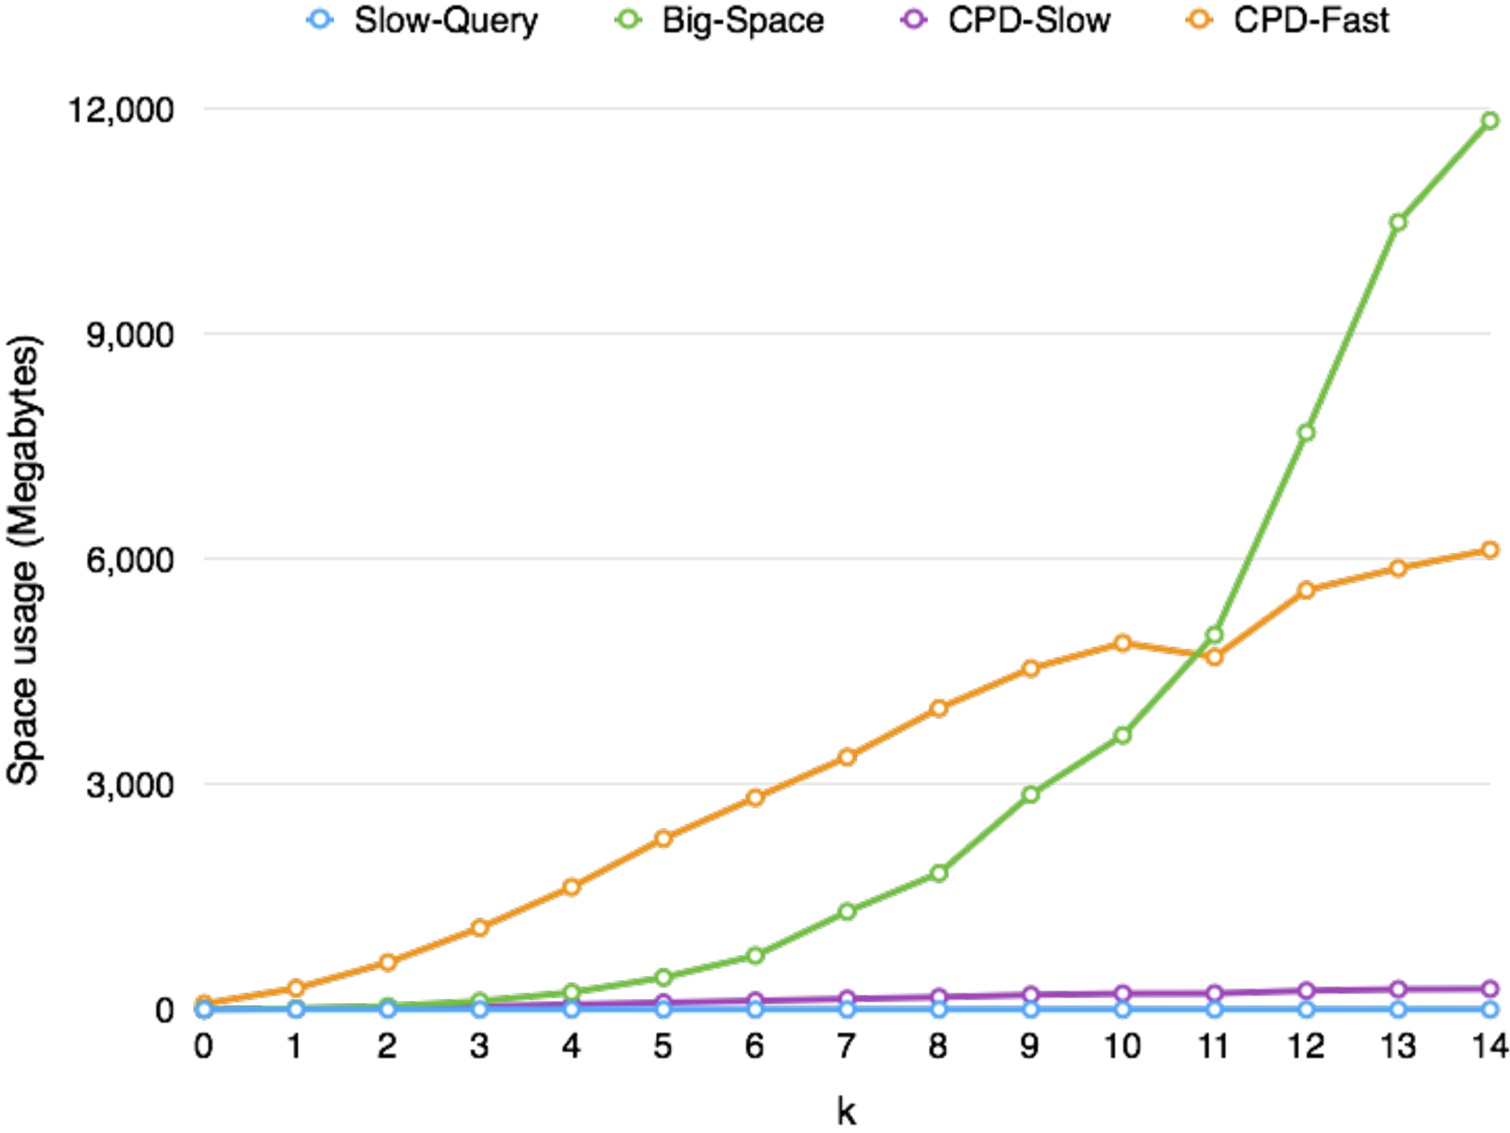
\includegraphics[height = 4in]{figures/plot-allfour-space.pdf}}
\end{center}
\caption{A space comparison of all four data structures. $t=5000$, $p=30$, and $k \in [0, 14]$.}
\label{fig:allfour-space}
\end{figure*}

\begin{figure*}[!t]
\begin{center}
\fbox{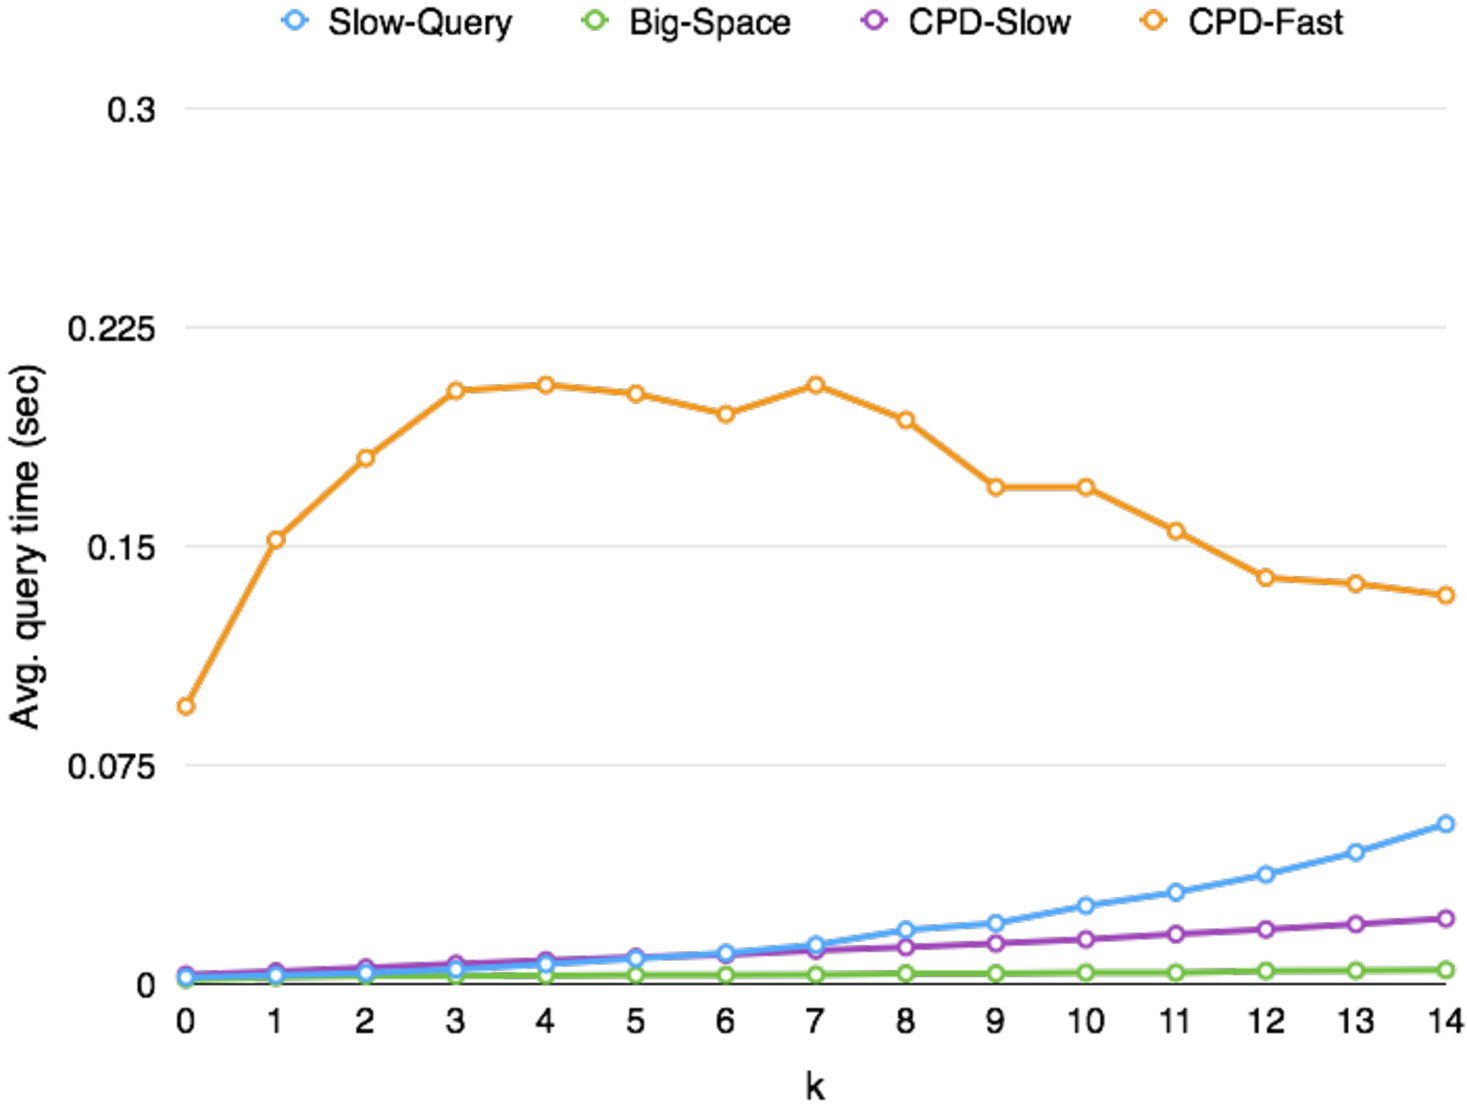
\includegraphics[height = 4in]{figures/plot-allfour-time.pdf}}
\end{center}
\caption{A runtime comparison of all four data structures. $t=5000$, $p=30$, and $k \in [0, 14]$.}
\label{fig:allfour-time}
\end{figure*}

We then seek to plot space usage and runtime individually for each of the data structures, where we now vary both $t$ and $k$.
For each experiment we again chose a fixed $p$, and a range of values for $t$ and $k$ that allow us to construct the data structures and run queries in a reasonable time.
Plots of the space usage for each of the four solutions are in Figures \ref{fig:space1}, \ref{fig:space2}, \ref{fig:space3}, and \ref{fig:space4}.
Plots of the average query running time for each of the four solutions are in Figures \ref{fig:time1}, \ref{fig:time2}, \ref{fig:time3}, and \ref{fig:time4}.

\section{Discussion}
\label{sec:discussion}

In this section we discuss the results of each of our experiments.
The primary discussion relevant to this paper is in the comparison of the four structures: Section~\ref{subsec:spacecompare} and Section~\ref{subsec:timecompare}.
The remaining discussion briefly explains the results of the experiments for each individual data structure.

\subsection{Space comparison of all four structures}
\label{subsec:spacecompare}

The space comparison of all four data structures, shown in Figure~\ref{fig:allfour-space}, fits well with what we expect from theory.
Indeed, the space usage of the \textsc{Slow-Query} data structure is small and has no dependence on $k$, as expected.
The space usage of the \textsc{CPD-Slow} data structure is also small and has a dependence on $k$, which is expected because the tree is grown recursively down to a depth of $k$ wildcards.
The space usage of the \textsc{CPD-Fast} structure is, for small $k$, the largest of the four approaches; this is most likely a consequence of the substantial overhead incurred by storing at each wildcard subtree all of the data structures necessary for performing LCP queries.
However, the space usage of the \textsc{Big-Space} structure ultimately exceeds the other structures and clearly grows exponentially in $k$, as expected.

\subsection{Query time comparison of all four structures}
\label{subsec:timecompare}

The average query time comparison of all four structures, shown in Figure~\ref{fig:allfour-time}, does not fit as closely with what we would expect from the theoretical bounds on runtime, but can be explained in practice.
Note that the growth and ordering of query times on the \textsc{Slow-Query}, \textsc{Big-Space}, and \textsc{CPD-Slow} structures are indeed in accordance with what we would expect from theory.

However, the query time on the \textsc{CPD-Fast} structure is surprising.
In particular, it is slower than the others (namely, slower than \textsc{Slow-Query} and \textsc{CPD-Slow}).
We believe it is slower than the other structures for two reasons.
First, there is substantial overhead, in terms of constant factors, incurred in performing LCP queries; this overhead is a part of the \textsc{CPD-Fast} structure, but not the \textsc{CPD-Slow} structure.
Second, we can compare the asymptotic runtimes of queries on the \textsc{CPD-Fast} structure and the \textsc{CPD-Slow} structure.
A query on the \textsc{CPD-Fast} structure runs in $O(p + 2^k \log \log t)$ time and a query on the \textsc{CPD-Slow} structure runs in $O(2^k p)$ time.\footnote{For clarity, in the remainder of the discussion we will omit the ``$+ \text{\# match}$'' from the asymptotic runtime.}
Hence, we would only expect queries on the \textsc{CPD-Fast} structure to be faster than those on the \textsc{CPD-Slow} structure if, roughly speaking, $\log \log t$ is smaller than $p$.
However, for the values of $t$ and $p$ we use (as well as for any reasonable choices), there is not a substantial difference between these values (i.e., they are within a factor of about 10).

Additionally, the plot for the query time on the \textsc{CPD-Fast} structure is surprising because the query time decreases as $k$ increases.
Our suspected reason for this is as follows:
When encountering a wildcard in a query pattern we perform a LCP query on a node at the root of a LCP structure and when encountering non-wildcard characters we perform an LCP query on a node which is not necessarily at the root of an LCP structure.
An unrooted LCP query has additional overhead and reduces to a rooted LCP query.
Therefore, in terms of constant factors, an unrooted LCP query should be strictly slower than a rooted LCP query.
As the number of wildcards in our queries increases, we perform more rooted LCP queries and fewer unrooted LCP queries, and thus the query time may begin to decrease.

\begin{figure}[ht]
\centering
\subfigure[{\textsc{Slow-Query} with $t$ from $100000$ to $900000$, $p = 100$, $k \in [0, 50]$}]{%
\fbox{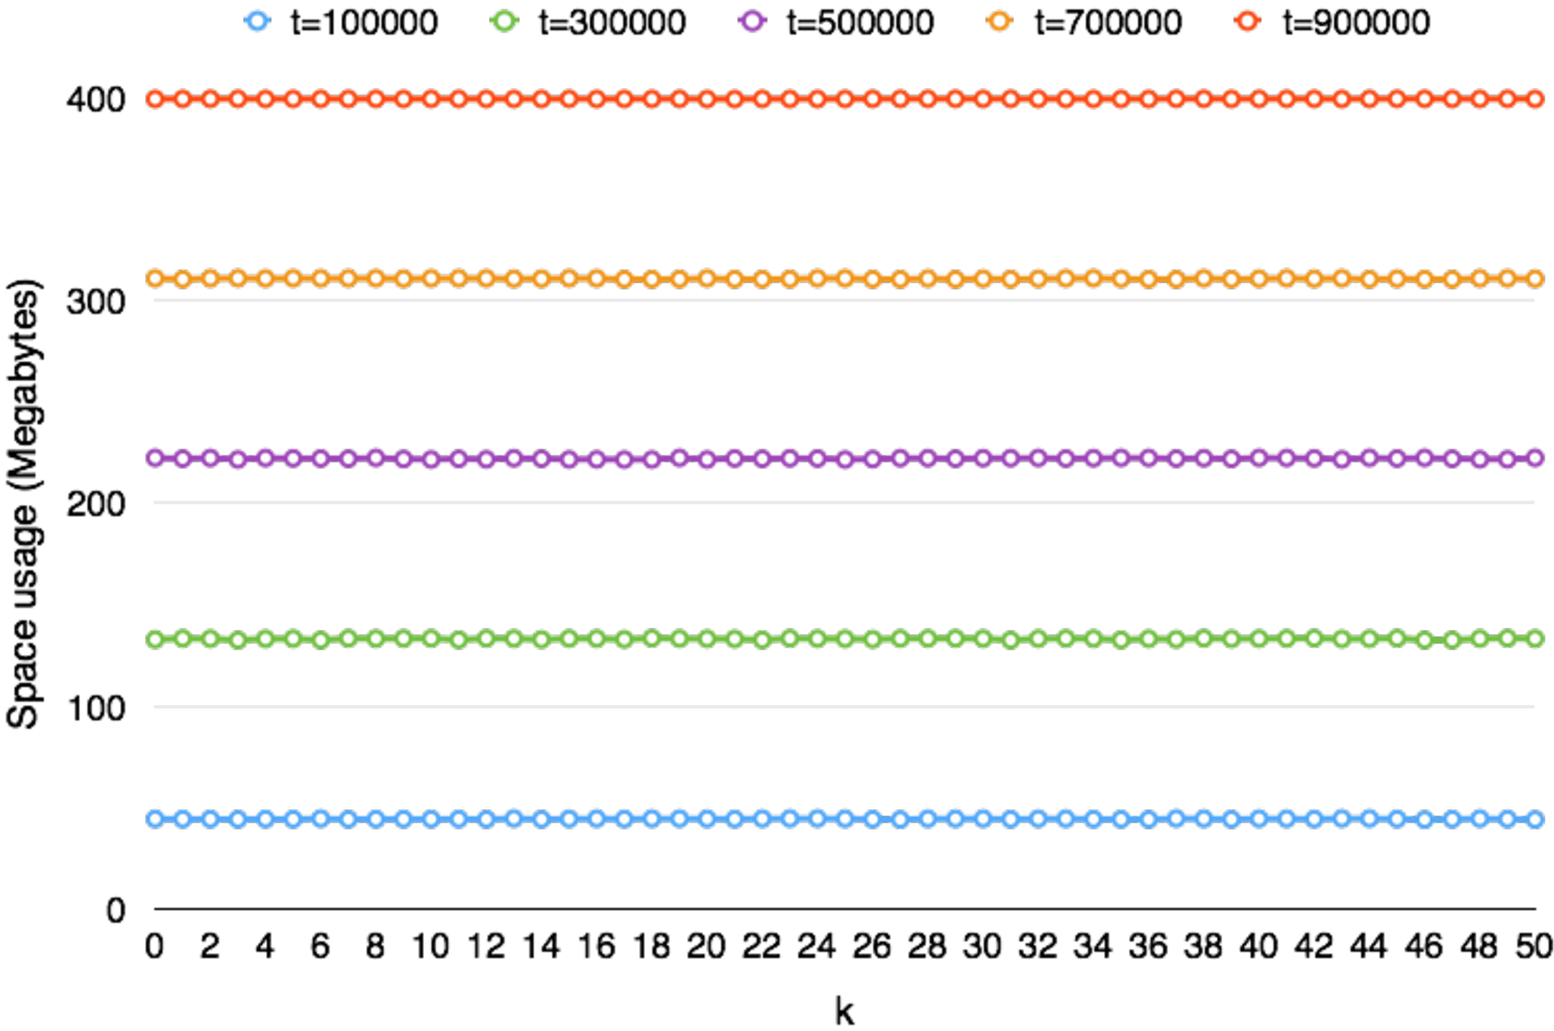
\includegraphics[width = 3in]{figures/plot-slowquery-space.pdf}}
\label{fig:space1}}
\quad
\subfigure[{\textsc{Big-Space} with $t$ from $2000$ to $10000$, $p = 25$, $k \in [0, 12]$}]{%
\fbox{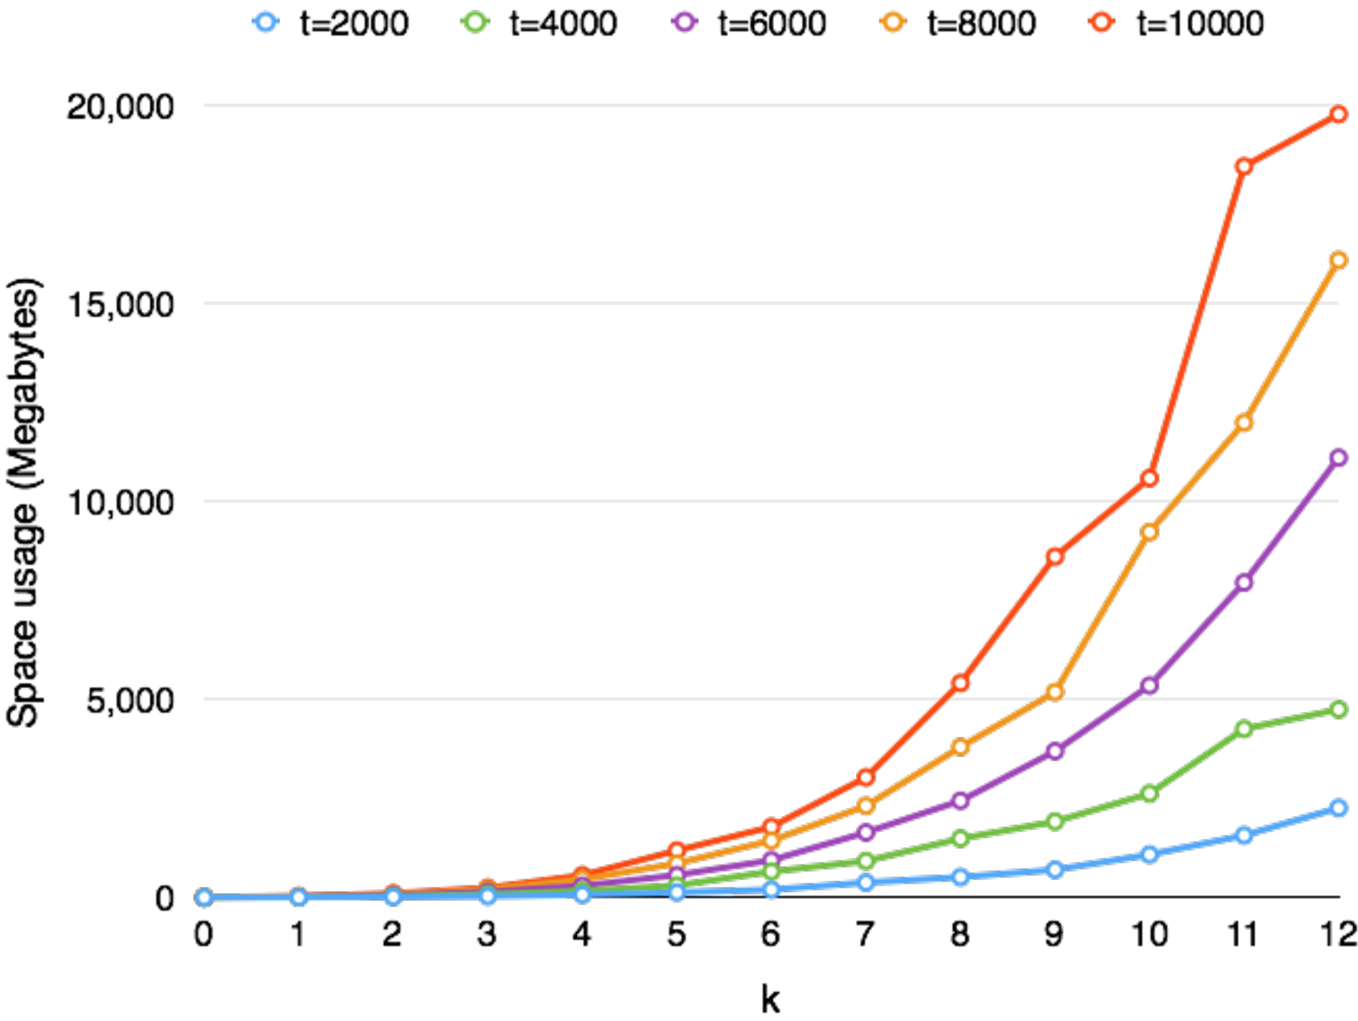
\includegraphics[width = 3in]{figures/plot-bigspace-space.pdf}}
\label{fig:space2}}
\subfigure[{\textsc{CPD-Slow} with $t$ from $4000$ to $20000$, $p = 30$, $k \in [0, 14]$}]{%
\fbox{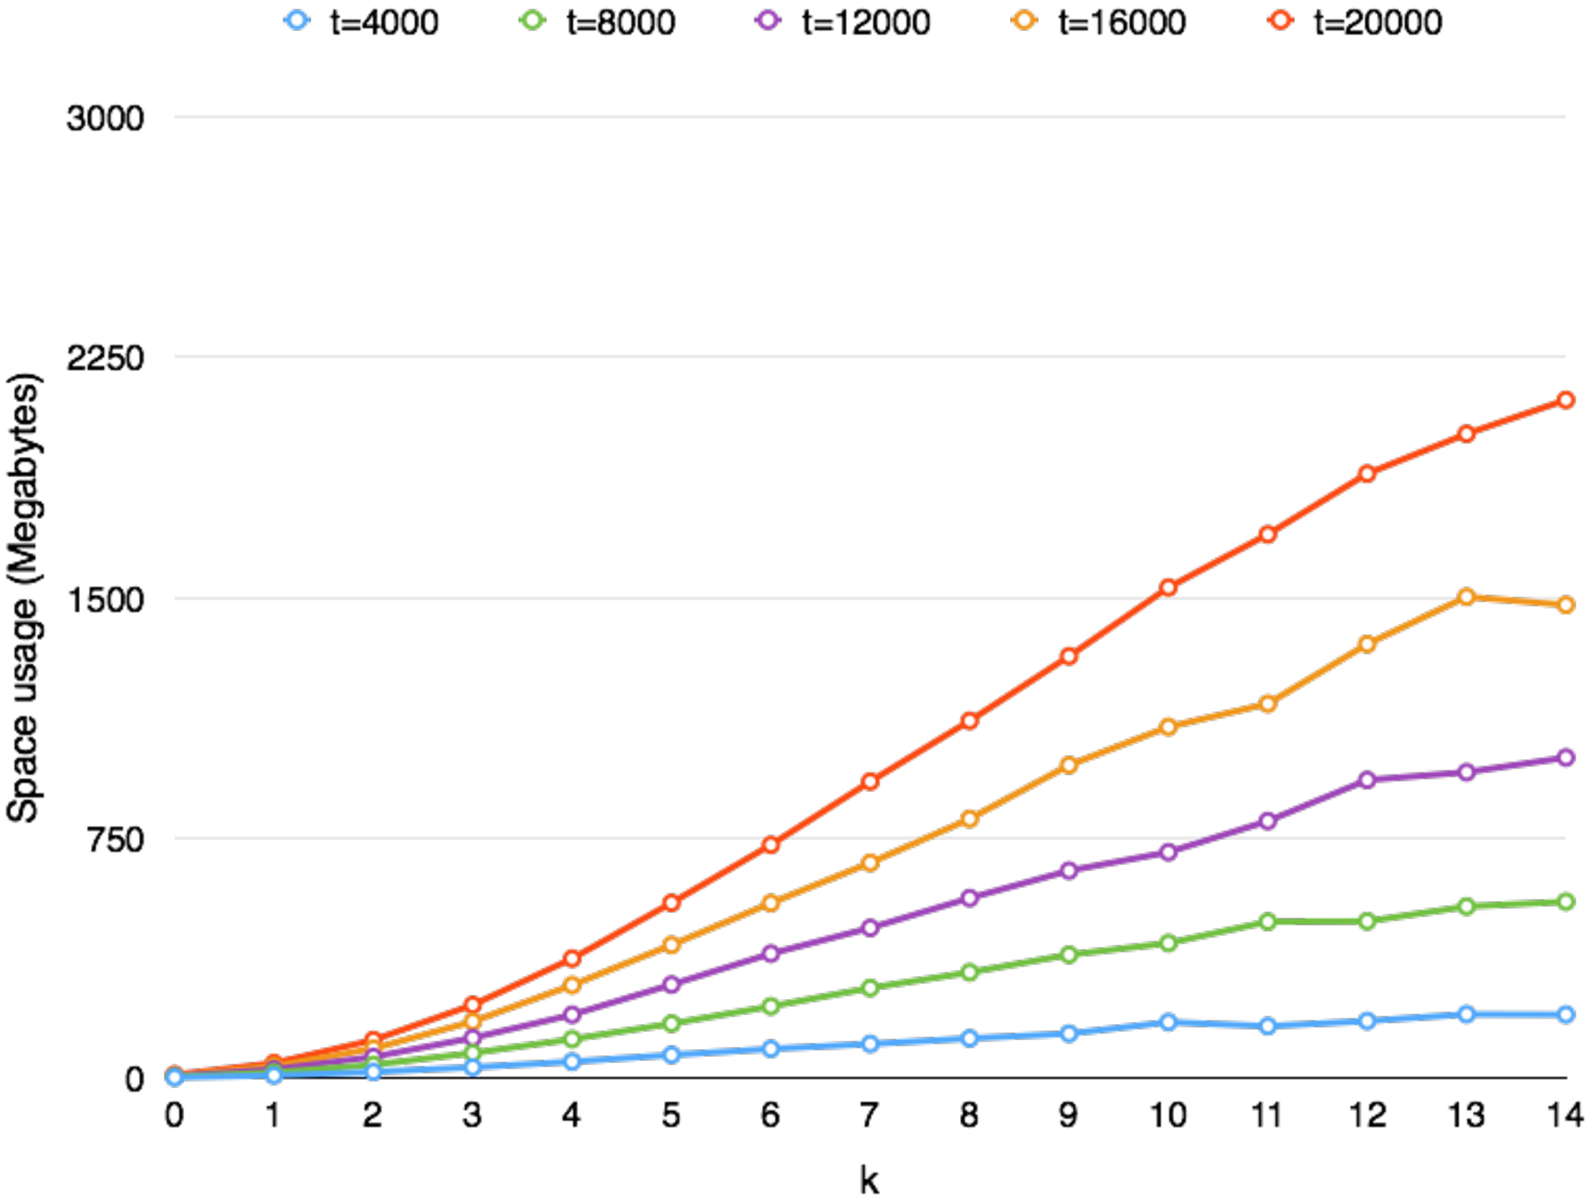
\includegraphics[width = 3in]{figures/plot-cpdslow-space.pdf}}
\label{fig:space3}}
\quad
\subfigure[{\textsc{CPD-Fast} with $t$ from $2000$ to $10000$, $p = 25$, $k \in [0, 12]$}]{%
\fbox{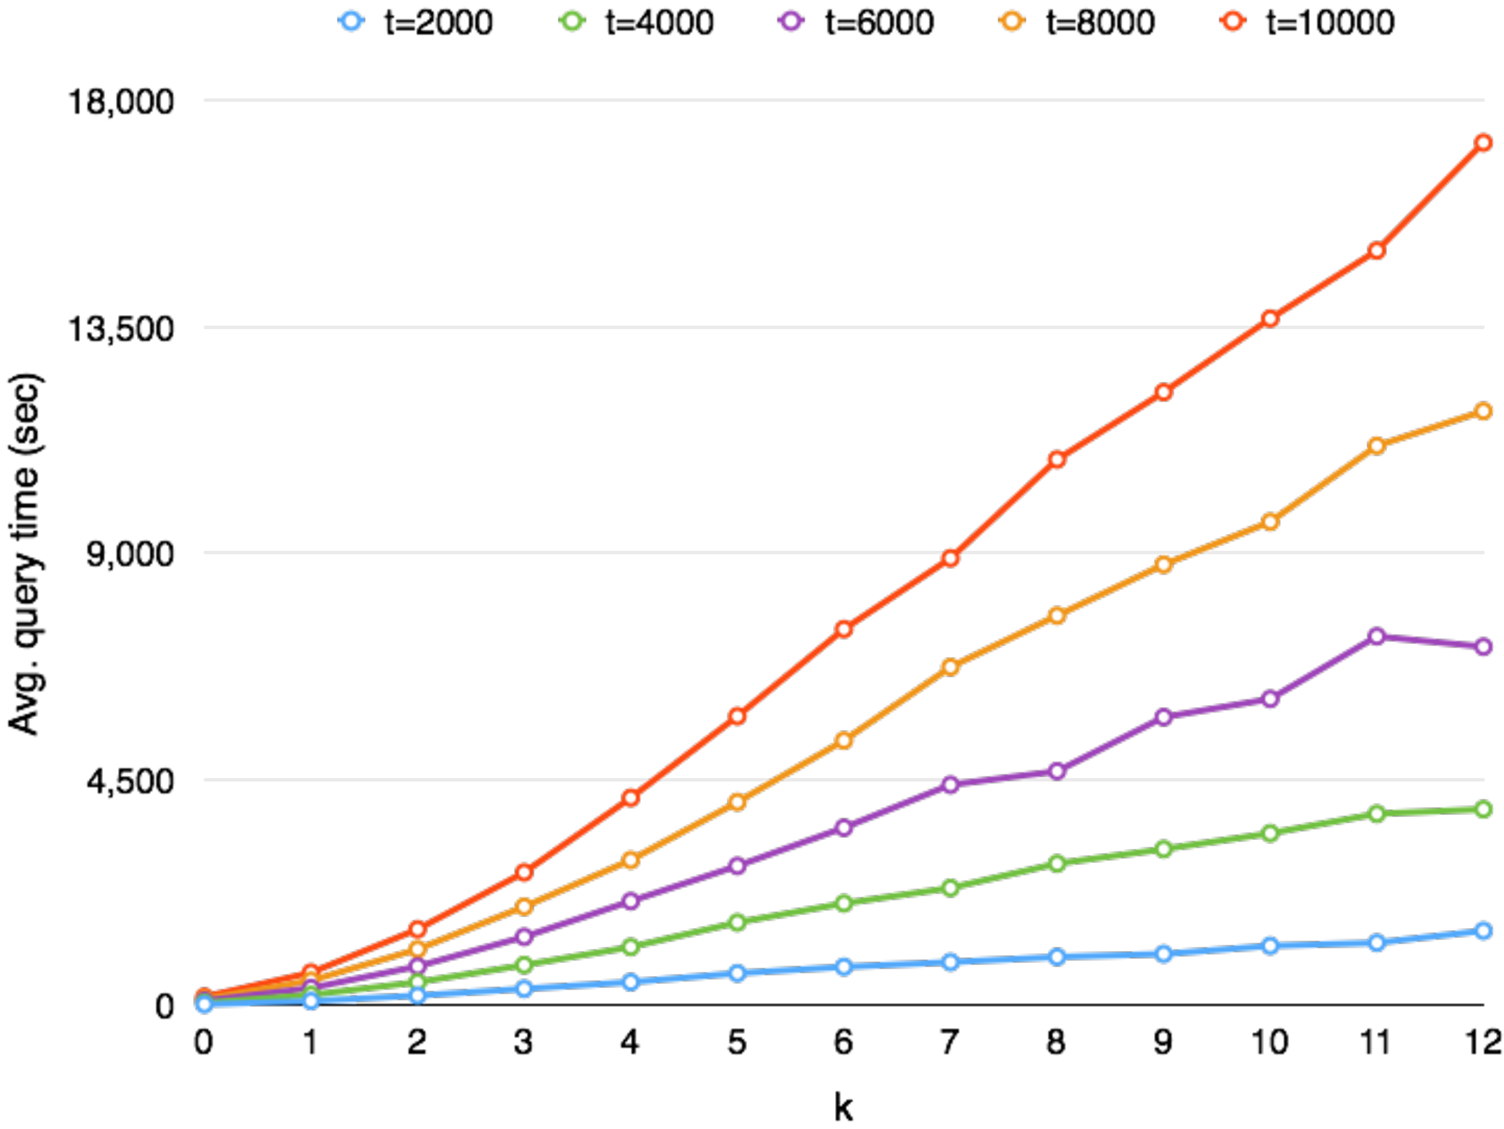
\includegraphics[width = 3in]{figures/plot-cpdfast-space.pdf}}
\label{fig:space4}}
%
\caption{The space usage of each of the different solutions for varying values of $t$ and $k$.}
\label{fig:figure}
\end{figure}

\begin{figure}[ht]
\centering
\subfigure[{\textsc{Slow-Query} with $t$ from $100000$ to $900000$, $p = 100$, $k \in [0, 50]$}]{%
\fbox{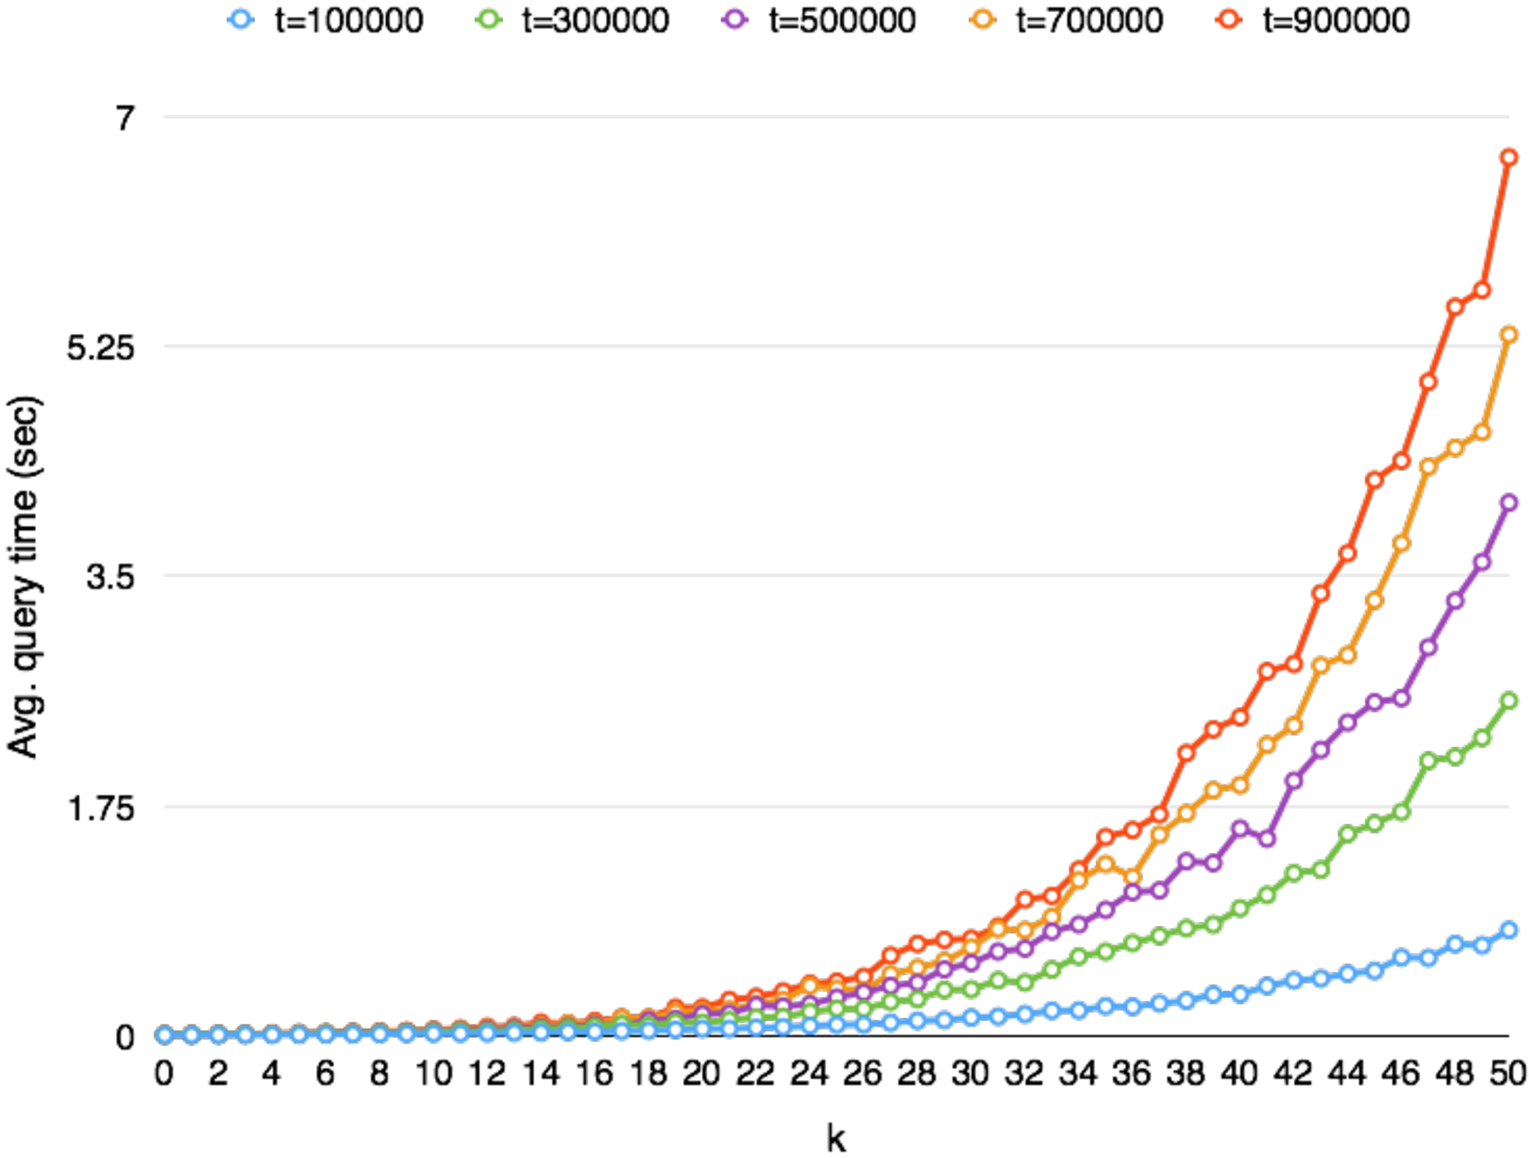
\includegraphics[width = 3in]{figures/plot-slowquery-time.pdf}}
\label{fig:time1}}
\quad
\subfigure[{\textsc{Big-Space} with $t$ from $2000$ to $10000$, $p = 25$, $k \in [0, 12]$}]{%
\fbox{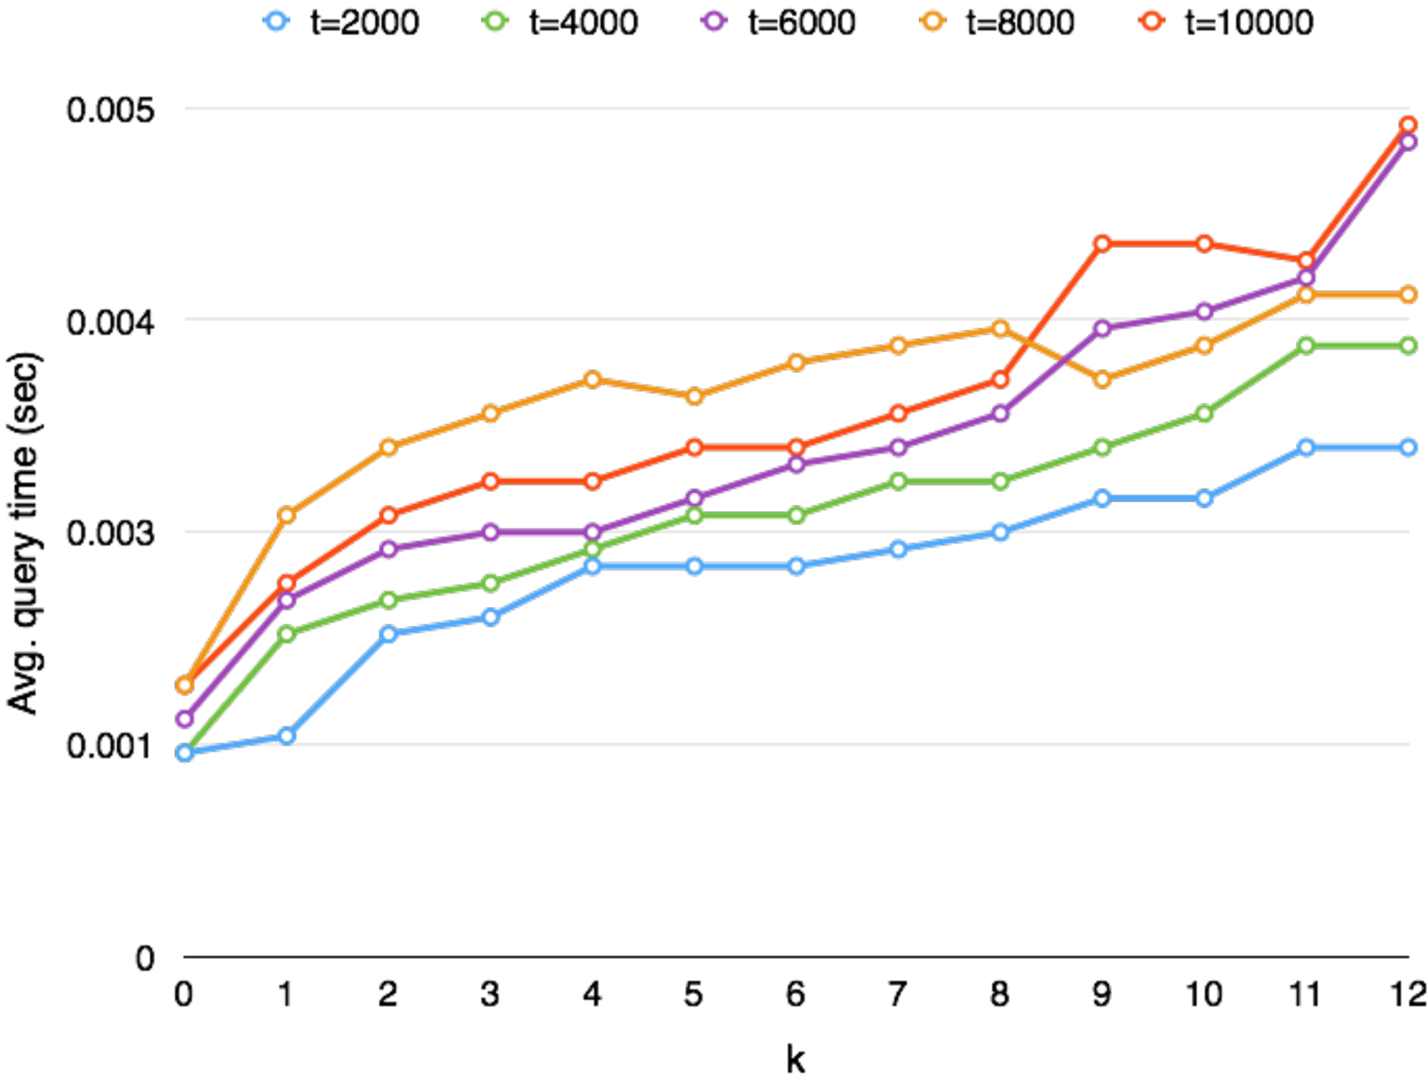
\includegraphics[width = 3in]{figures/plot-bigspace-time.pdf}}
\label{fig:time2}}
\subfigure[{\textsc{CPD-Slow} with $t$ from $4000$ to $20000$, $p = 30$, $k \in [0, 14]$}]{%
\fbox{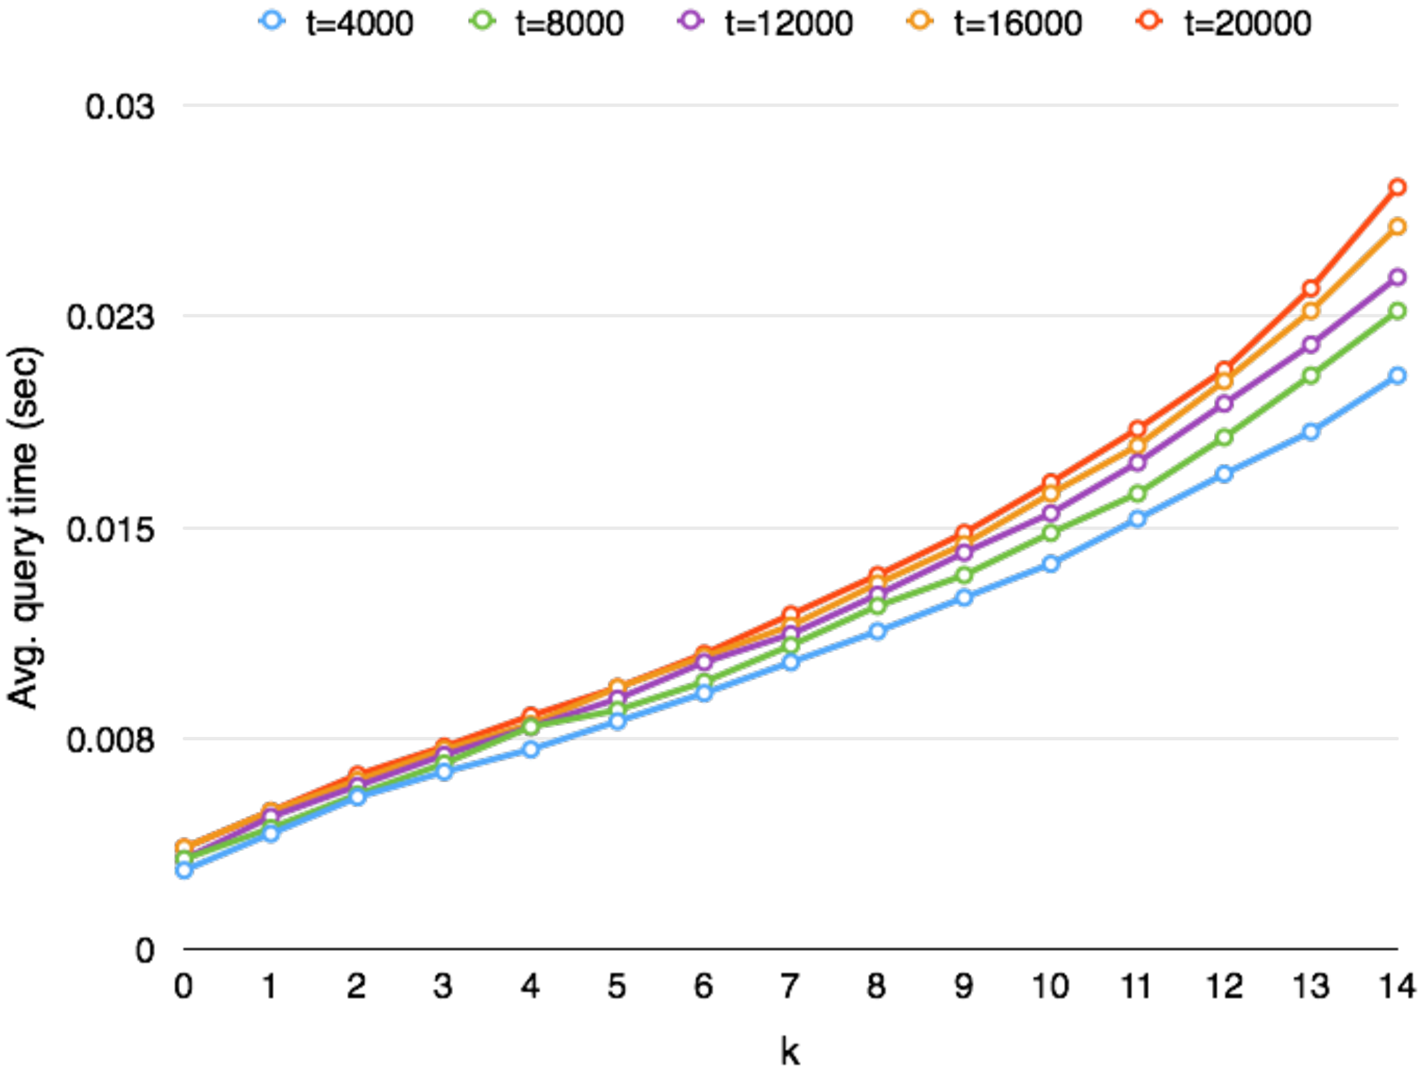
\includegraphics[width = 3in]{figures/plot-cpdslow-time.pdf}}
\label{fig:time3}}
\quad
\subfigure[{\textsc{CPD-Fast} with $t$ from $2000$ to $10000$, $p = 25$, $k \in [0, 12]$}]{%
\fbox{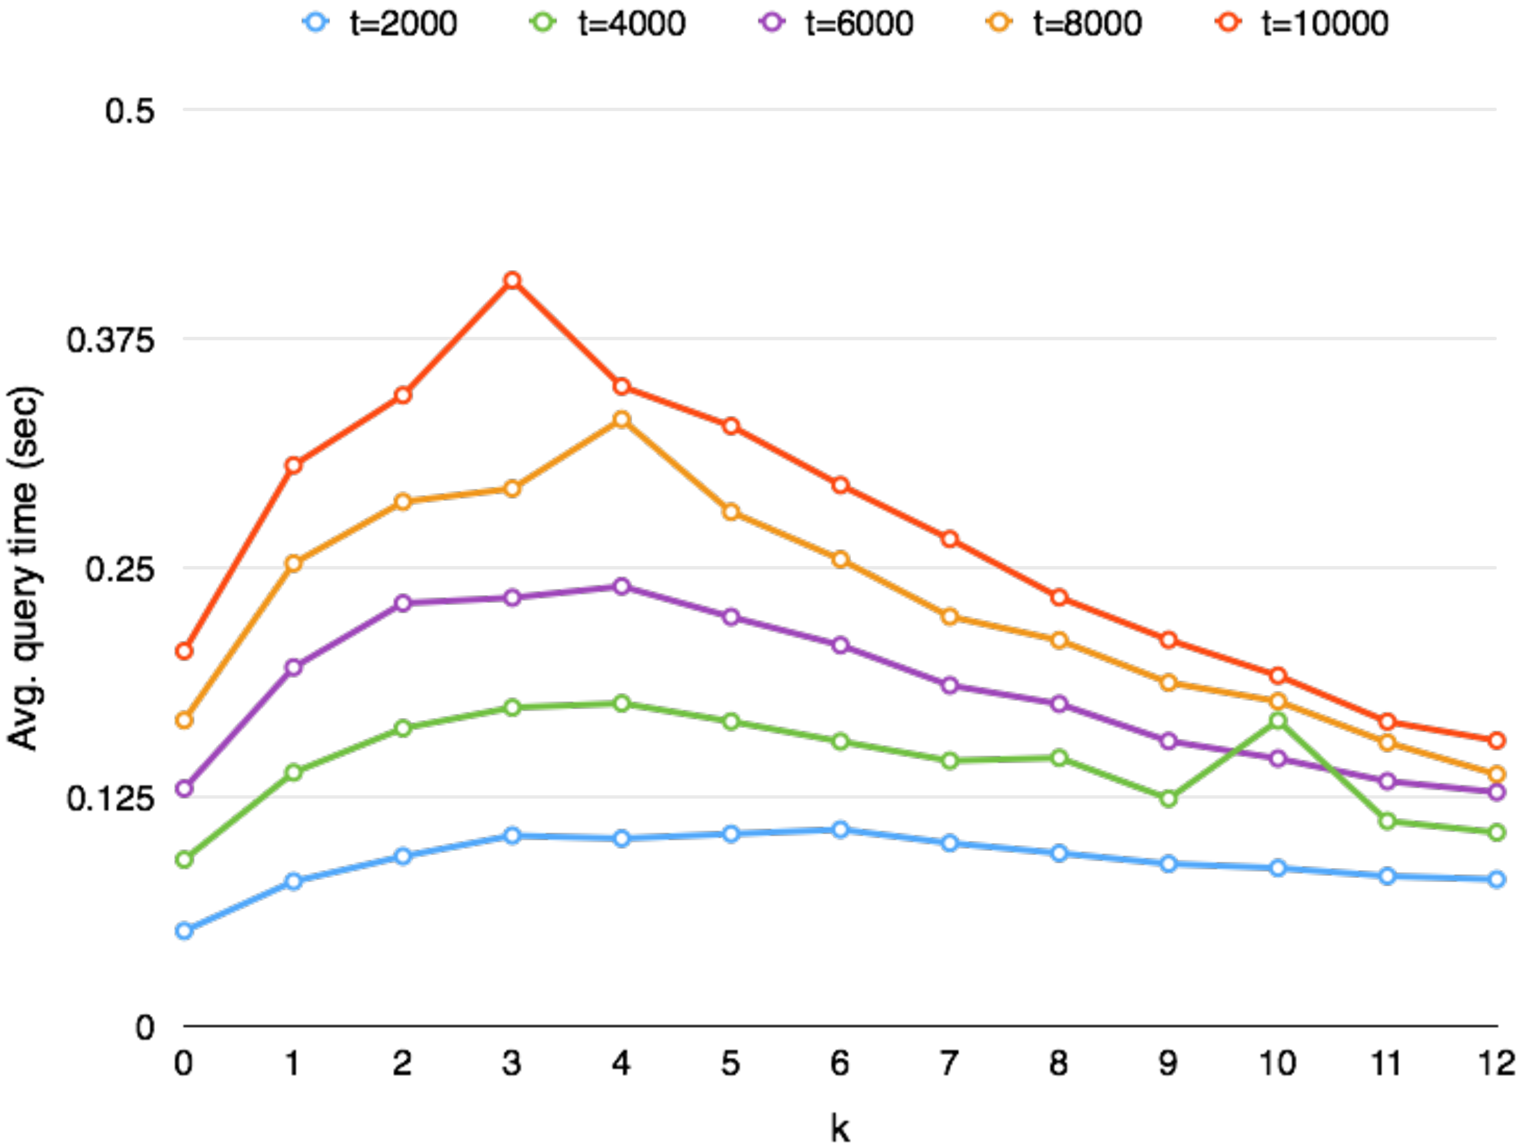
\includegraphics[width = 3in]{figures/plot-cpdfast-time.pdf}}
\label{fig:time4}}
%
\caption{The average query time of each of the different solutions for varying values of $t$ and $k$.}
\label{fig:figure}
\end{figure}

\subsection{Space and time of the \textsc{Slow-Query} structure}

The \textsc{Slow-Query} solution behaved as expected based on asymptotic runtimes for both space usage and query time. In Figure~\ref{fig:space1}, we can see that the total space has no dependence on $k$ (as expected), and also that the total space increases in equally spaced increments as we increase $t$ by the same amount. In Figure~\ref{fig:time1}, we see that the query time depends exponentially on $k$. This matches our runtime of $O(\Sigma^kp)$. While the runtime does not directly depend on $t$, a larger value of $t$ means there are more possible occurrences of the query text, and therefore more branching occurs when searching for the query. Thus, we observe that the query time increases as $t$ increases.

\subsection{Space and time of the \textsc{Big-Space} structure}

The \textsc{Big-Space} solution also behaved as expected for both space usage and query time. We see in Figure~\ref{fig:space2} that space usage increases exponentially with $k$ and also increases for increasing $t$. In Figure~\ref{fig:time2}, we see that the query time has very little dependence on $k$, which is expected from the $O(p)$ runtime. The slight upward trend can be explained by the fact that we only decide to search along a wildcard edge once we have checked all the other edges and found no match; therefore, when we have more wildcards, we have to iterate through more edges, so the runtime increases slightly.

\subsection{Space and time of the \textsc{CPD-Slow} structure}
The \textsc{CPD-Slow} solution similarly produced reasonable plots. First, in Figure~\ref{fig:space3} we can see that the space usage increases with $k$ and $t$. The increase in space as we increase $k$ is not quite as exponential as we might have expected from the $O(t\log^k{t})$ space analysis, although from \cite{cole} we can see that this bound is not perfectly tight. Thus, the space performance is actually better than anticipated. In Figure~\ref{fig:time3} we see that the query time is exponential in $k$, as expected, with only a small dependence on $t$.

\subsection{Space and time of the \textsc{CPD-Fast} structure}
The \textsc{CPD-Fast} solution produced the most surprising results. In Figure~\ref{fig:space4}, we see that the space usage is not unexpected. The plot looks very similar to that of that for \textsc{CPD-Slow}, with a slightly steeper slope that is probably caused by the fact that we have to store much more information with this solution. The surprising plot is that in Figure~\ref{fig:time4}, because we see that the query time actually decreases as we increase $k$. A possible explanation for this was offered in Section~\ref{subsec:timecompare}.

\section{Conclusion}

We find that the naive approaches (\textsc{Slow-Query} and \textsc{Big-Space}) perform as expected from theory in both space usage and query time.
The analysis of the solutions proposed by Cole et al. (\textsc{CPD-Slow} and \textsc{CPD-Fast}) is more involved.
In particular, the \textsc{CPD-Slow} structure outperforms the \textsc{CPD-Fast} structure in both space usage and in query time for practical parameter values.
We speculated on reasons for this.
Furthermore, the \textsc{CPD-Slow} structure has a space usage roughly similar to that of the \textsc{Slow-Query} structure (i.e., very small) and a query time that lies between the times required by the \textsc{Big-Space} and the \textsc{Slow-Query} structures.
Hence, we conclude that, among the four approaches with which we experimented, the \textsc{CPD-Slow} approach offers the optimal compromise between space and time.

 \begin{thebibliography}{9}
\bibitem{cole}
Richard Cole, Lee-Ad Gottlieb, and Moshe Lewenstein.
 Dictionary matching and indexing with errors and don't cares.
 In \textit{Proc. 36th ACM Symposium on Theory of Computing (STOC)},
 pages 91--100, 2004.
 
 \bibitem{lec}
 Erik Demaifne. Least Common and Level Ancestors. MIT 6.851 Lectures 15 Notes Spring 2014. http://courses.csail.mit.edu/6.851/spring14/lectures/L15.pdf
 
 \bibitem{ukkonenstackoverflow}
 StackOverflow. \textit{Ukkonen's suffix tree algorithm in plain English?} March 2012 --- May 2013. http://stackoverflow.com/questions/9452701/ukkonens-suffix-tree-algorithm-in-plain-english/
 
 \bibitem{ukkonengithub}
 Max Garfinkel, GitHub. \textit{A java implementation of Ukkonen's suffix tree creation algorithm.} September 2012. https://github.com/maxgarfinkel/suffixTree/
 
 \bibitem{cuckoo}
 Keith Schwarz. \textit{Cuckoo-Hashmap.} November 2010 --- December 2013. https://github.com/maxgarfinkel/suffixTree/
 
 \bibitem{oanc}
 The Open American National Corpus. http://www.anc.org/data/oanc/
 
 \bibitem{memorymeter}
 Jonathan Ellis. \textit{Java Agent for Memory Measurements.} February 2011 --- May 2014. https://github.com/jbellis/jamm
\end{thebibliography}

\end{document}
